\chapter{Application}\label{sensor-application}
In this chapter the sensor application will be presented. 
Several sequence diagrams will be explained, as well as concepts needed to understand the flow of the application. 

\section{Health Sensors}
There is an ongoing discussion of when the health technology revolution will come to human bodies now that \gls{IoT} have become so popular.
By revolution, I mean sensors placed in the human body. 
Sensors that can read your blood pressure, heart rate and measure insulin levels.
Sensors that can detect whether your body is missing out of a substance, or if its poisoned. 
There is no limit for what can be done.
Everything that should be measured, will be measured by sensors integrated in the human body.
But who will be able to read the data?
Or perform instructions to the sensors/devices?
There is some major privacy issues related to this discussion, and there problems that needs to be solved.

In 2011, Jerome Radcliffe discovered that his insulin pump easily could be hacked~\cite{radcliffe2011hacking}.
Basically the pump would take instructions from anyone and do anything, with no questions asked. 
This is a worst case scenario when it comes to hacking medical devices attached to a human.

For this matter I propose a health sensor system that is built upon \gls{NDN} with \gls{IBC} ensuring a secure and locked environment.
First, let me introduce you to The Stig. 
He has developed diabetes and as everybody else that do not have diabetes, he does not want to manually monitor his glucose levels and adjust the insulin pump at every meal. 
He has injected a \gls{CGM} to monitor his glucose levels and report to the insulin pump, automatically.
In addition to his diabetes, he has a heart disease which forces him to monitor his heart rate at any given time. 
In~\autoref{fig:health-sensor-system} we can see The Stig with all his sensors and devices. 
The \gls{CGM} reports periodically to the insulin pump, and all sensors reports to The Stig's mobile so that The Stig can watch what is going on.

\begin{figure}[ht]
  \centering
  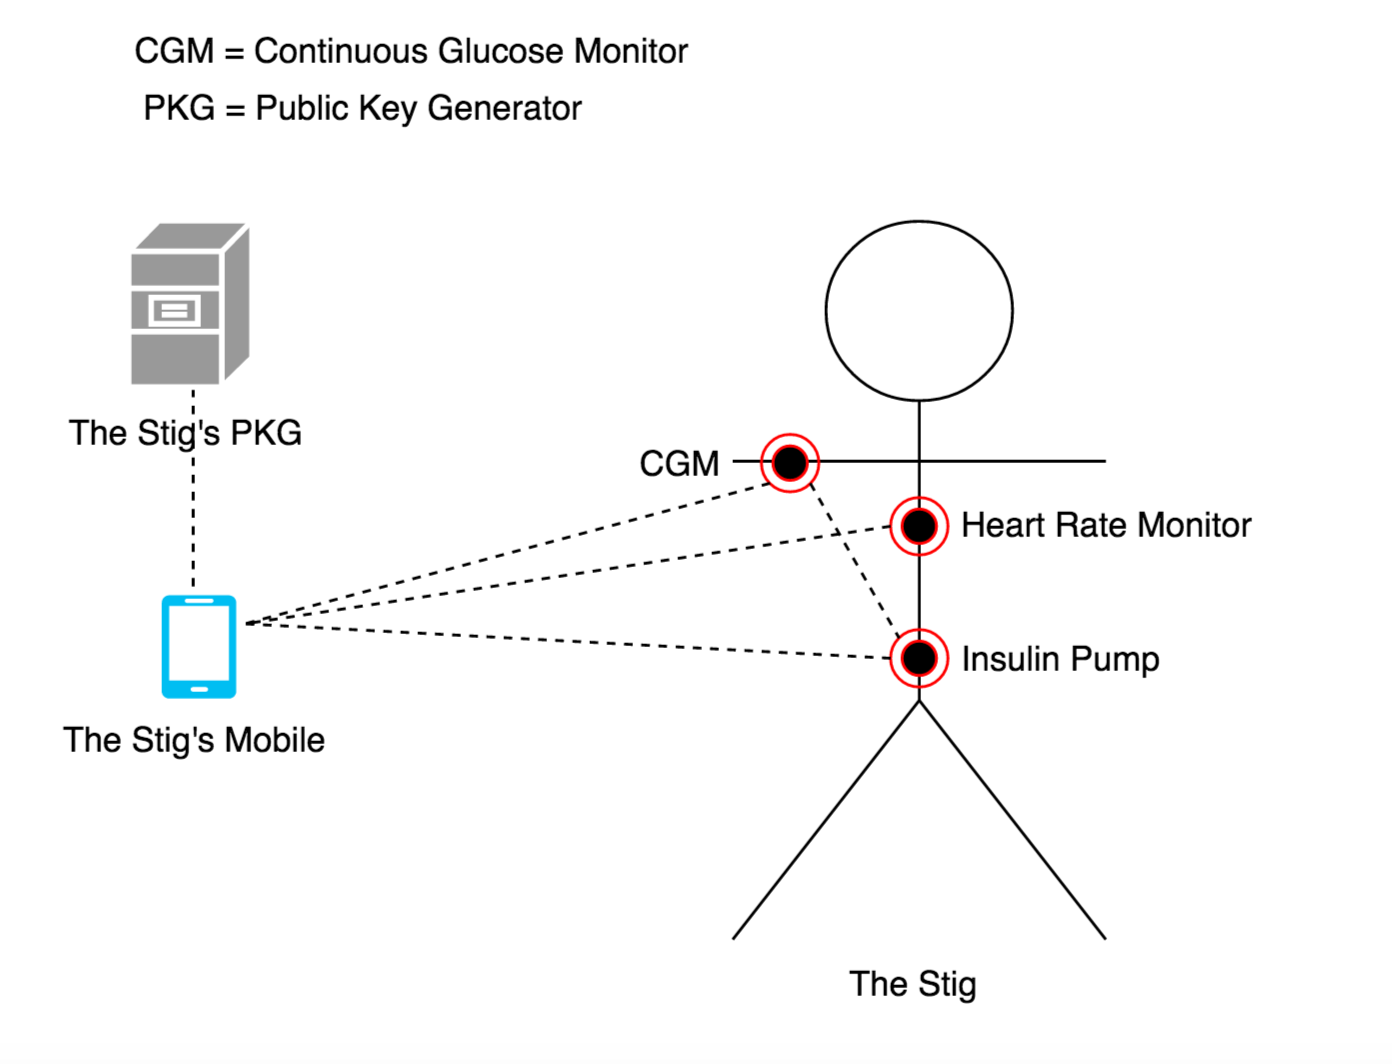
\includegraphics[width=1\textwidth]{health-sensor-system.png}
  \caption{Health Sensor System}
  \label{fig:health-sensor-system}
\end{figure}

\section{Health Sensor System}\label{hss}
To have a secure system, it needs to be established trust between the sensors and the devices.
There needs to be integrity controls, confidentiality protection and access control. 
In the following sections, I will describe the protocols suggested for achieving the mentioned goals.

\subsection{Rendezvous Authentication}\label{rendezvous_authentication}
One of the best solutions for authentication of an identity in cryptography is rendezvous authentication, the concept of meeting face-to-face for authenticating who you are talking to. 
In \gls{IoT}, we have in most cases the advantage of identifying devices in a physical matter. 
This means that it is possible to authenticate devices, such as sensors. 
Typically, this kind of authentication will rely on 1) manually inspection and 2) digital connection, e.g. through \gls{NFC}.
In the proposed system, I assume that this type of authentication is achieved in a secure matter and do not discuss whether how this should be done.

\subsection{Initialization}
When The Stig is setting up his health sensor system, first he wants to configure the \gls{PKG}. 
Any type of computer can play the role of the \gls{PKG} and The Stig has chosen his home server, from now ``the PKG''.
The \gls{PKG} creates two key pairs that is used to do \gls{IBE} and \gls{IBS}.
Second, he wants his mobile device, from now ``the mobile'', to be a part of the \gls{PKG}s trust domain, and further add all of the other devices and sensors, from now ``device(s)''.

\begin{enumerate}
  \item First device, e.g. a mobile, connects to the \gls{PKG} through physical connection as showed in~\autoref{fig:init_ibe_1}.
  \item Additional devices can connect through physical connection via another authorized device, or the \gls{PKG} itself. 
  \item Data pulling from existing nodes in network~\autoref{fig:data_pull_ibe}
\end{enumerate}

In~\autoref{fig:init_ibe_1} the device acts as the mobile. 
The \gls{ID} of every device has been given the term Name, this is due to \gls{NDN}. 
Hence \gls{ID} and Name is the same.
To be able to communicate securely under initialization, the device have to create a temporary \gls{MPK} and \gls{MSK} and then extract a temporary Private Key for its Name. 
At first, the device has to act as a \gls{PKG} for itself to ensure confidentiality, and the trust between the device and the real \gls{PKG} is based on the concept explained in~\autoref{rendezvous_authentication}.
The device sends an Interest appending the temporary \gls{MPK} and the Name to the \gls{PKG} asking to join the \gls{PKG}s domain.
The \gls{PKG} encrypts a \gls{CEK} with the temporary \gls{MPK} and the Name received from the device. 
Then the \gls{PKG} extracts the Private Key for the device (this will be the key belonging to the \gls{PKG}s trust domain) and uses the \gls{CEK} to do a symmetric \gls{AES} encryption on the Private Key. 
The Data packet response to the initialization Interest will contain the identity-based encrypted \gls{CEK}, the symmetric encrypted Private Key and the \gls{PKG}s \gls{MPK}.
To finish the initialization protocol, the device decrypts the \gls{CEK}, throws away the temporary keys, and finally decrypts the Private Key.
The device has established a trust with its \gls{PKG} and can verify other devices in this domain. 

Now that the mobile is authenticated, devices can connect to the mobile through e.g. \gls{NFC} for initialization.
This results in a rendezvous authentication between the device and the mobile, and if the mobile is given the authorities to perform initialization (\autoref{access_control}), the new device has joined the \gls{PKG}s trust domain.

\begin{figure}[ht]
  \centering
  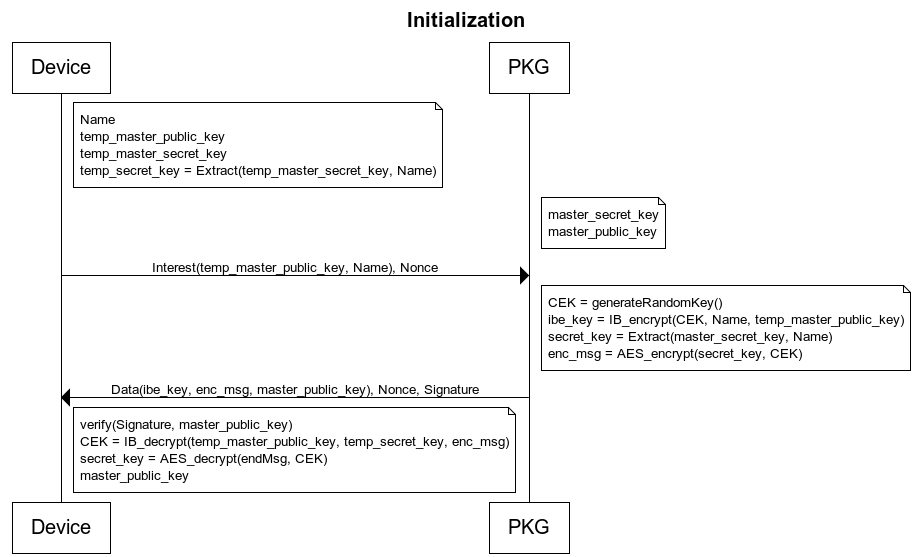
\includegraphics[width=1\textwidth]{Initialization.png}
  \caption{Initialization IBE}
  \label{fig:init_ibe_1}
\end{figure}



% \begin{figure}[ht]
%   \centering
%   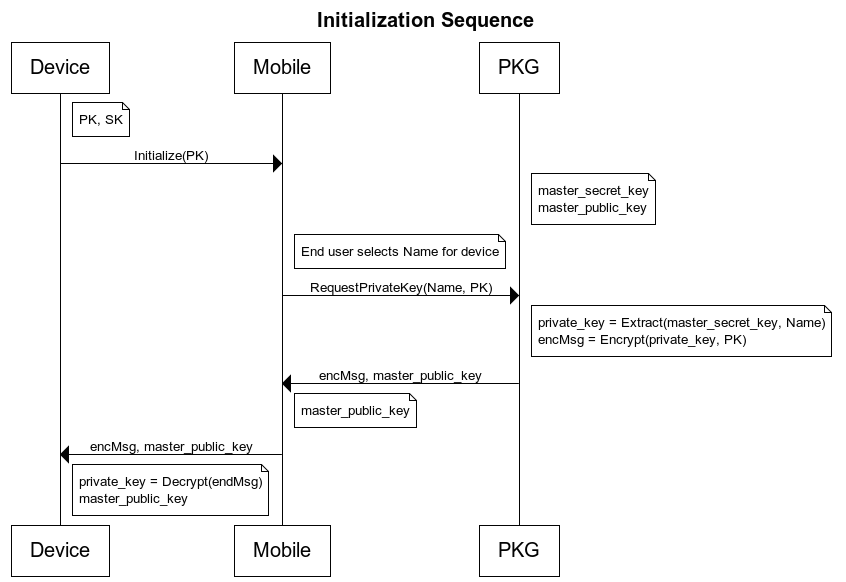
\includegraphics[width=1\textwidth]{init_ibe_2.png}
%   \caption{Initialization IBE through authorized device}
%   \label{fig:init_ibe_2}
% \end{figure}

% \begin{lstlisting}[language=BASH, caption={Initialization}, label={lst:ibe-initialization}]
% pkg = new PublicKeyGenerator;
% for device in {devices}
% do
% 	device -> connect to pkg;
% 	pkg -> verify device then issue Private Key;
% 	device -> subscribe Name Sync and Public Key
% done
% \end{lstlisting}

\subsection{Data Pull}
As illustrated in~\autoref{fig:health-sensor-system}, the devices has now joined the \gls{PKG}s trust domain and are ready to communicate.
This flow is illustrated in~\autoref{fig:data_pull_ibe}.
By signing the Interest and appending the Name, the receiving device can verify that the requester is a part of the same trust domain, and also be able to encrypt the sensor data (if needed) with the requesters Name.
The requesting device receives the Data and verifies the signature and decrypts the sensor data.

\begin{figure}[ht]
  \centering
  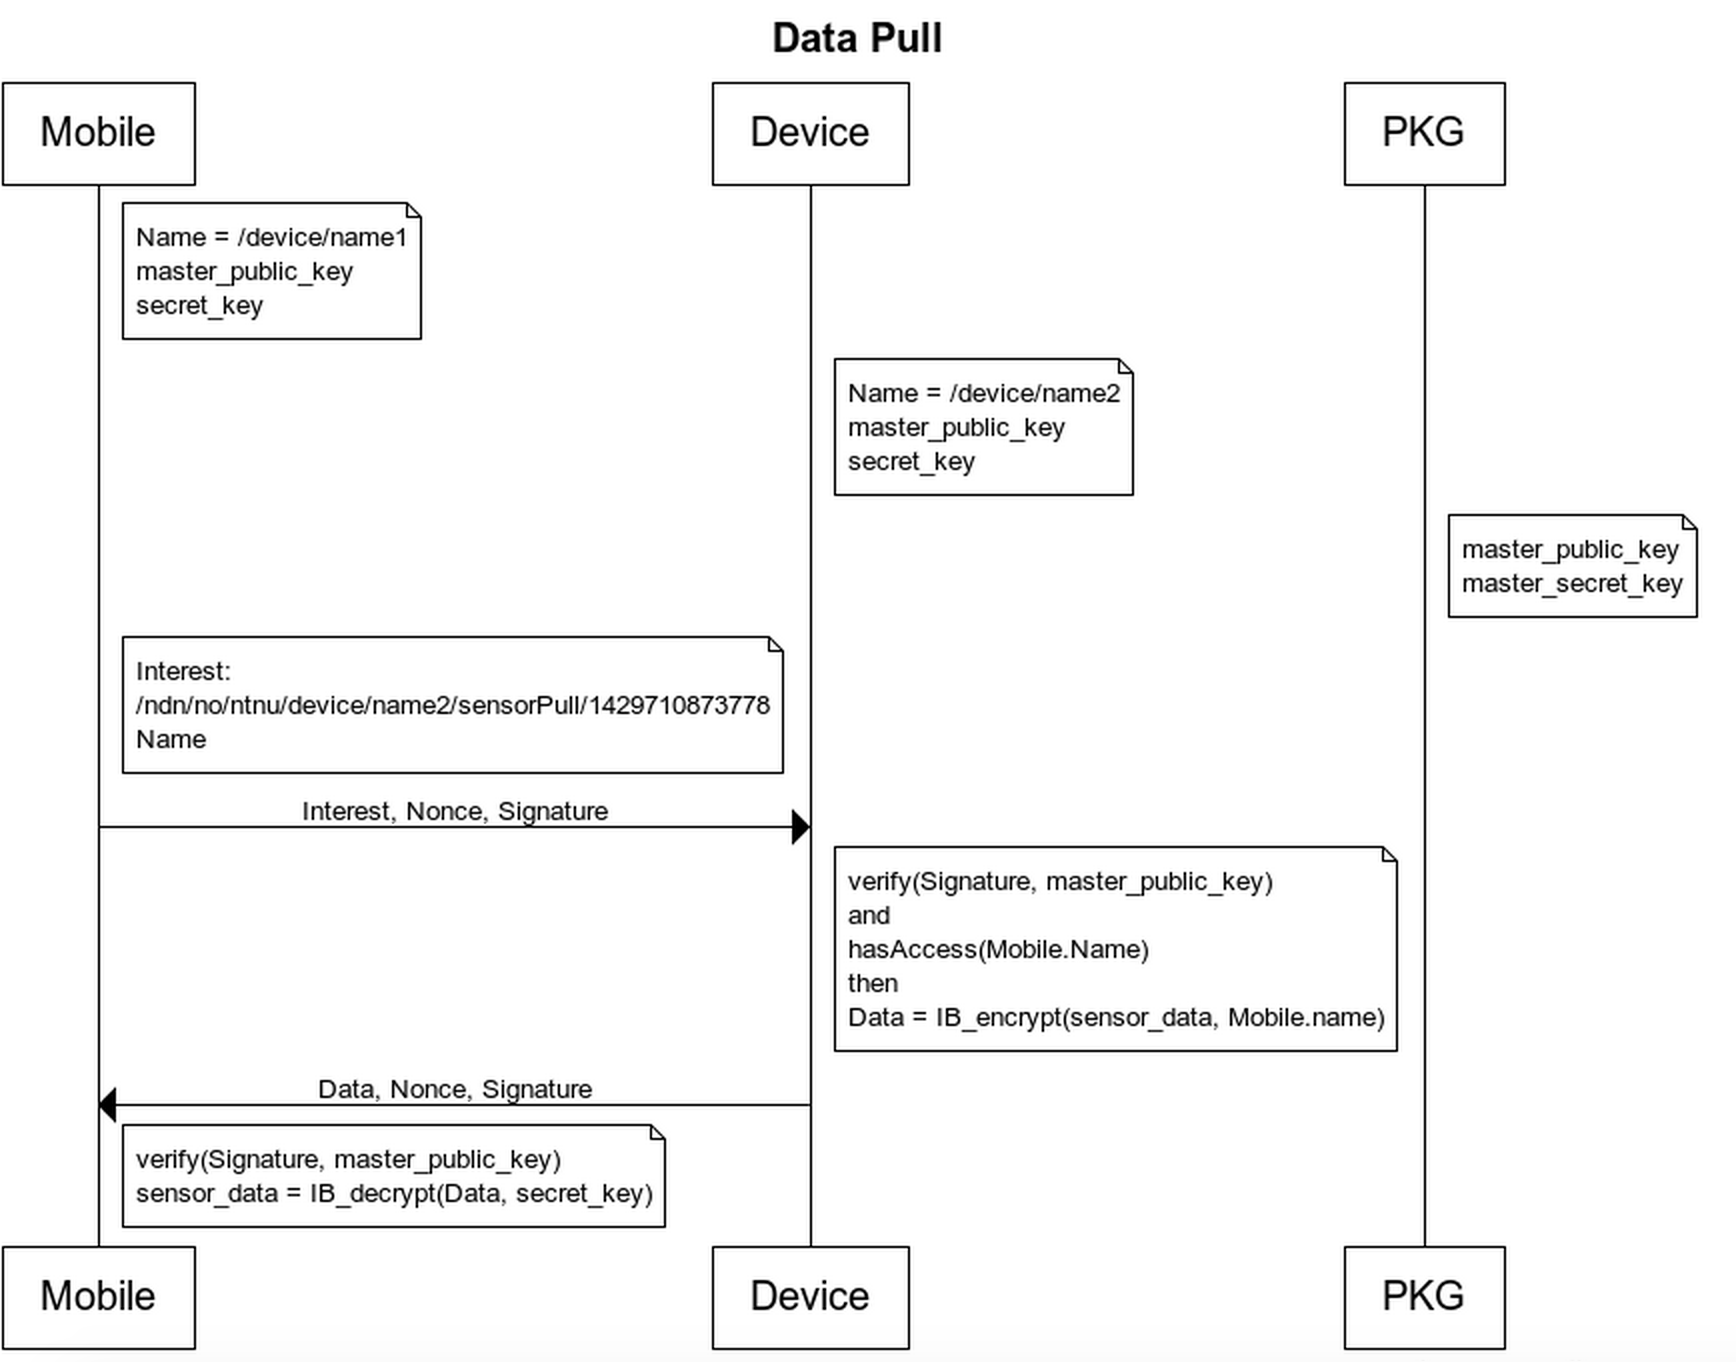
\includegraphics[width=1\textwidth]{DataPull.png}
  \caption{Mobile performing a data pull from a device in the network.}
  \label{fig:data_pull_ibe}
\end{figure}

\subsection{IDSync}
The File Synchronization Module (\autoref{file-sync}) can be used to distribute a fresh list of every device that is a member of the trust domain.
This synchronization will be controlled by the \gls{PKG}, hence every device can verify each synchronization message.

\section{Confidentiality, Integrity and Availability}
\subsection{Confidentiality}

All data can be, if needed, encrypted.
The encryption can be achieved by encrypting with the Name of the requester as the public key.


\subsection{Integrity and Authenticity}

Each device will obtain a private key allocated by its superior \gls{PKG}, as explained in~\autoref{ibc}.
With the concept from~\autoref{rendezvous_authentication} together with the \gls{PKG}s \gls{MPK}, you can trust that the device is authorized for the \gls{PKG}s network. Hence all signed packets can be verified by anyone with the \gls{MPK}.

\subsection{Replay Attack}
Every Interest has a timestamp attached to the Name (e.g. \path{/ndn/no/ntnu/device/name2/sensorPull/1429710873778}), i.e. milliseconds from \path{UTC 1970-01-01 00:00:00}, that is used for protection against replay attack. 


\subsection{Availability}

This is a harder problem to solve.
The network is purely wireless, hence vulnerable to jamming. 

\section{Trust Model}


\subsection{Access Control}\label{access_control}

When a device retrieves an Interest for its sensor data, there should be a authorization mechanism. 

Capability based approach to \gls{IoT} access control~\cite{DBLP:conf/imis/GusmeroliPR12}.

Least privilege access